\documentclass[runningheads]{llncs}
\usepackage[T1]{fontenc}
\usepackage[utf8]{inputenc}
\usepackage[spanish,es-tabla]{babel}
\usepackage{graphicx}
\usepackage{array}
\usepackage{booktabs}
\usepackage{xurl}
\usepackage[hidelinks]{hyperref}
\newcolumntype{L}[1]{>{\raggedright\arraybackslash}p{#1}}
\newcolumntype{C}[1]{>{\centering\arraybackslash}p{#1}}

% Cabeceras en el margen interno (lado del cosido); número de página en el margen externo
\makeatletter
\def\ps@headings{\let\@mkboth\@gobbletwo
  \let\@oddfoot\@empty\let\@evenfoot\@empty
  \def\@evenhead{\normalfont\small\rlap{\thepage}\hfil\leftmark}%  par: interno = derecha
  \def\@oddhead{\normalfont\small\rightmark\hfil\llap{\thepage}}%  impar: interno = izquierda
  \def\chaptermark##1{}\def\sectionmark##1{}\def\subsectionmark##1{}}
\makeatother
\pagestyle{headings}

\begin{document}

\title{Planificación de la producción de una bodega ante el Superniño 2026--2027: un plan redactado con asistencia de IA}
\titlerunning{Planificación de la producción ante el Superniño}

\author{Sara Kemelmajer \and Rocío Ana Martinez \and María Pilar Mujica \and Lucía Salamone}
\authorrunning{S. Kemelmajer et al.}

\institute{Universidad Nacional de Cuyo, Instituto de Ingeniería Industrial\\
\url{https://ingenieria.uncuyo.edu.ar/}}

\maketitle

\begin{abstract}
Este informe aplica la metodología de redacción asistida por inteligencia artificial propuesta en el primer informe del módulo a un caso del proyecto final: la planificación de la producción de una bodega ubicada en el parque industrial PASIP (Palmira, Mendoza) para la vendimia 2027, bajo el fenómeno de El Niño muy fuerte o ``Superniño'' previsto para 2026--2027. Se siguieron los cinco pasos de la metodología: se definió el contexto, se aportaron los datos propios de los módulos anteriores, se pidió el documento por partes, se verificó cada dato contra su fuente y se iteró. El diagnóstico se apoya en datos del Instituto Nacional de Vitivinicultura: en 2016, con el Niño anterior, la cosecha de Mendoza cayó cerca de un 45\,\%. Con esa referencia se plantearon tres escenarios de abastecimiento y un plan agregado de recepción semanal de uva. El resultado principal es que el escenario más exigente para la planta no es el de mayor caída de volumen, sino uno moderado: la cosecha se concentra en menos semanas y la selección sanitaria reduce la capacidad efectiva, de modo que se superaría la capacidad en dos semanas (480\,t). Se proponen un segundo turno, contratos de abastecimiento alternativo, un cronograma de preparación y una matriz de riesgos. Todos los parámetros de la planta son supuestos del equipo y están identificados como tales.

\keywords{UNCUYO \and TyHM \and Superniño \and Planificación de la producción \and Inteligencia artificial.}
\end{abstract}

\section{Introducción}

En el Módulo 1 el equipo eligió, con herramientas de toma de decisiones, el fenómeno del Superniño como tema de un capítulo del proyecto final, orientado a la planificación de la producción agroindustrial. En el Módulo 3 se estudió con sistemas de información geográfica el riesgo hídrico de los parques industriales de Mendoza ante El Niño \cite{sig}, y en la continuación con SQL se decidió, con el método AHP, ubicar la planta en el parque PASIP de Palmira (San Martín) \cite{sql}. En el primer informe de este módulo se propuso una metodología para redactar planes y proyectos con asistencia de IA \cite{informeia}.

Este informe une esas piezas. Tiene dos objetivos: (1) redactar el plan de producción de la planta para la vendimia 2027 ante el Superniño, y (2) mostrar en un caso real cómo se aplican los cinco pasos de la metodología y qué controles exige cada sección.

\section{Metodología de redacción con IA}

Se siguieron los cinco pasos propuestos en el primer informe \cite{informeia}. La Tabla~\ref{tab:pasos} resume cómo se aplicó cada uno.

\begin{table}
\caption{Aplicación de los cinco pasos de la metodología.}\label{tab:pasos}
\centering
\begin{tabular}{L{2.8cm}L{8.6cm}}
\toprule
\textbf{Paso} & \textbf{Cómo se aplicó en este informe}\\
\midrule
1. Definir el contexto & Se indicó el tipo de documento (plan de producción), el destinatario (cátedra y proyecto final), el formato (LNCS) y el tono (técnico).\\
2. Aportar los datos propios & Se entregaron los resultados de los Módulos 1 y 3 y de la continuación SQL: tema elegido, riesgo hídrico por parque y localización en el PASIP.\\
3. Pedir por partes & Se redactó una sección por vez, en el orden de la estructura estándar de un plan: diagnóstico, objetivos, alcance, plan, cronograma, presupuesto y riesgos.\\
4. Revisar críticamente & Cada cifra se verificó contra su fuente (Tabla~\ref{tab:verificacion}) y los parámetros sin fuente se marcaron como supuestos.\\
5. Iterar & Se corrigieron secciones puntuales; por ejemplo, al agregar la pérdida de capacidad por selección sanitaria cambió el escenario crítico (Sección~\ref{sec:plan}).\\
\bottomrule
\end{tabular}
\end{table}

La instrucción de contexto con la que se inició el trabajo, resumida, fue la siguiente:

\begin{verbatim}
Actuá como ingeniero industrial. Redactá un plan de producción
para una bodega ubicada en el PASIP (Palmira, Mendoza) para la
vendimia 2027, ante el Superniño 2026-2027. Usá los datos de
nuestros módulos anteriores (riesgo hídrico por parque, decisión
de localización). Seguí la estructura: diagnóstico, objetivos
SMART, alcance, plan, cronograma, presupuesto y riesgos. No
inventes cifras: usá fuentes verificables o marcá los supuestos.
Formato LNCS, tono formal.
\end{verbatim}

Según la tabla de aplicaciones del primer informe, las secciones de diagnóstico, cronograma y riesgos requieren revisión alta, y el presupuesto, muy alta \cite{informeia}. Por eso, en el presupuesto la IA solo propuso la estructura, sin valores.

\section{Diagnóstico}

\subsection{El Superniño 2026--2027}

En agosto de 2026 la NOAA elevó a cerca del 95\,\% la probabilidad de que El Niño sea muy fuerte (anomalía superior a 2\,$^\circ$C) entre octubre y diciembre; la semana del 5 de agosto la anomalía en la región Niño 3.4 ya era de $+1{,}8\,^\circ$C, la más temprana de la serie \cite{noaa}. La NOAA estima en 97\,\% la probabilidad de que el fenómeno se mantenga hasta comienzos de 2027 \cite{smn}.

Para Mendoza, el Servicio Meteorológico Nacional asignó entre 50 y 55\,\% de probabilidad a lluvias superiores a lo normal para agosto--octubre, con tormentas fuertes aisladas \cite{smn}. Según el IANIGLA, se esperan más nevadas en la cordillera y mayor ocurrencia de tormentas severas en verano \cite{ianigla}. El trabajo del Módulo 3 es coherente con esto: en años Niño la precipitación invernal en la cordillera aumenta un 22\,\% y la superficie potencialmente inundable del piedemonte pasa de 258 a 425\,km$^2$ \cite{sig}.

\subsection{El antecedente de 2016}

El Niño 2015--2016 es la referencia más cercana. Las lluvias persistentes favorecieron enfermedades fúngicas de hojas y racimos, la pérdida de hojas redujo la acumulación de azúcar, y el granizo agravó los daños; en el Este y el Norte de Mendoza la vid cayó alrededor de un 40\,\% \cite{freshplaza}. La Tabla~\ref{tab:cosecha} compara las cosechas.

\begin{table}
\caption{Uva cosechada o elaborada en Mendoza y en el país (millones de quintales).}\label{tab:cosecha}
\centering
\begin{tabular}{L{3.6cm}C{1.6cm}C{1.6cm}C{1.6cm}C{1.6cm}}
\toprule
 & \textbf{2015} & \textbf{2016} & \textbf{2025} & \textbf{2026}\\
\midrule
Mendoza & 16{,}81 & 9{,}24 & 15{,}04 & 13{,}18\\
Total del país & 23{,}90 & 15{,}39 & 19{,}51 & 18{,}39\\
\bottomrule
\end{tabular}

\medskip
\footnotesize Fuentes: 2015, dato preliminar del INV al 7/5/2015 \cite{inv2015}; 2016, 2025 y 2026, uva elaborada según el informe final de cosecha 2026 del INV \cite{inv2026}.
\end{table}

Entre 2015 y 2016 la cosecha de Mendoza bajó cerca de un 45\,\% y la del país un 36\,\%. San Juan fue la única provincia que cosechó más que el año anterior \cite{sanjuan}, lo que muestra que el abastecimiento desde otra región puede compensar parte de la caída. La vendimia 2026 ya fue un 12\,\% menor que la de 2025 en Mendoza \cite{inv2026}, por lo que la planta parte de un año de oferta reducida.

\subsection{Análisis FODA}

La Tabla~\ref{tab:foda} resume la situación de la planta frente al fenómeno.

\begin{table}
\caption{Matriz FODA de la planta frente al Superniño.}\label{tab:foda}
\centering
\begin{tabular}{L{5.7cm}L{5.7cm}}
\toprule
\textbf{Fortalezas} & \textbf{Debilidades}\\
\midrule
Ubicación en el PASIP, elegida por menor riesgo hídrico y cercanía a la materia prima \cite{sql}. & Abastecimiento concentrado en el Este, la zona más afectada en 2016.\\
Pronóstico disponible con meses de anticipación. & Capacidad de recepción ajustada al pico de un año normal.\\
\midrule
\textbf{Oportunidades} & \textbf{Amenazas}\\
\midrule
Más nieve: mayor disponibilidad de agua de riego en el verano \cite{ianigla}. & Lluvias y granizo en la maduración; enfermedades fúngicas.\\
Uva de otras regiones (San Juan) menos afectada en 2016 \cite{sanjuan}. & Caída de volumen y aumento del costo fijo por tonelada.\\
\bottomrule
\end{tabular}
\end{table}

\section{Objetivos}

\textbf{Objetivo general.} Asegurar que la planta procese toda la uva disponible en la vendimia 2027 con la calidad sanitaria requerida, en cualquiera de los escenarios del Superniño.

\textbf{Objetivos específicos (SMART).}
\begin{enumerate}
\item Mantener en menos de 24\,h el tiempo entre la cosecha y la molienda del 100\,\% de la uva recibida durante toda la vendimia 2027.
\item Firmar antes del 31/01/2027 contratos de abastecimiento alternativo, fuera del Este de Mendoza, por al menos 2.400\,t (20\,\% del volumen de un año normal).
\item Tener listo antes del 15/02/2027 un segundo turno que aumente la capacidad semanal en un 30\,\%.
\item Terminar el mantenimiento preventivo de la línea de recepción y molienda antes del 31/01/2027.
\end{enumerate}

\section{Alcance}

El plan comprende la recepción, la selección sanitaria y la molienda de la uva en la planta del PASIP entre febrero y abril de 2027, y la preparación previa desde noviembre de 2026. No incluye el manejo de los viñedos de los proveedores, la fermentación y crianza posteriores, ni la comercialización del vino.

\section{Plan de producción}\label{sec:plan}

\subsection{Supuestos}

La IA no conoce los datos reales de una planta, por lo que se definieron los supuestos de la Tabla~\ref{tab:supuestos}. Las proporciones semanales siguen una forma de campana típica de la vendimia; en los escenarios Niño la cosecha se comprime porque se adelanta la uva con riesgo de podredumbre.

\begin{table}
\caption{Supuestos del plan (definidos por el equipo).}\label{tab:supuestos}
\centering
\begin{tabular}{L{6.6cm}L{4.8cm}}
\toprule
\textbf{Parámetro} & \textbf{Valor supuesto}\\
\midrule
Uva contratada en un año normal & 12.000\,t\\
Capacidad nominal de recepción y molienda & 320\,t/día, 6 días: 1.920\,t/semana\\
Pérdida de capacidad por selección sanitaria & 15\,\%: 1.632\,t/semana\\
Duración de la vendimia normal & 10 semanas\\
Caída de volumen, Niño moderado & 20\,\%, en 8 semanas\\
Caída de volumen, Superniño & 45\,\% (como 2016), en 7 semanas\\
\bottomrule
\end{tabular}
\end{table}

\subsection{Escenarios}

La Fig.~\ref{fig:recepcion} muestra la recepción semanal en cada escenario y la Tabla~\ref{tab:escenarios} resume los indicadores. El plan sigue el enfoque de planeación agregada de la bibliografía de operaciones \cite{heizer}; los cálculos se hicieron con el script en Python incluido con el informe.

\begin{figure}
\centering
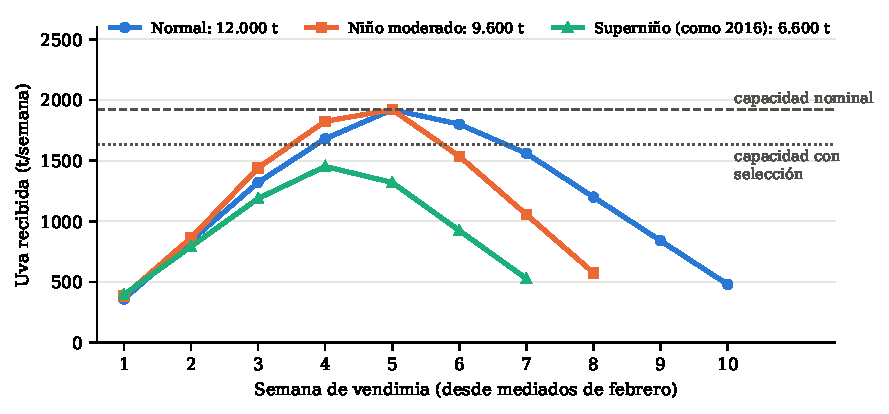
\includegraphics[width=\textwidth]{recepcion_semanal.pdf}
\caption{Recepción semanal de uva en los tres escenarios y capacidad de la planta.}
\label{fig:recepcion}
\end{figure}

\begin{table}
\caption{Indicadores del plan agregado por escenario.}\label{tab:escenarios}
\centering
\begin{tabular}{L{3.9cm}C{2.4cm}C{2.4cm}C{2.4cm}}
\toprule
\textbf{Indicador} & \textbf{Normal} & \textbf{Niño moderado} & \textbf{Superniño}\\
\midrule
Uva recibida (t) & 12.000 & 9.600 & 6.600\\
Semanas de vendimia & 10 & 8 & 7\\
Pico semanal (t) & 1.920 & 1.920 & 1.452\\
Capacidad efectiva (t/semana) & 1.920 & 1.632 & 1.632\\
Uso de capacidad en el pico & 100\,\% & 118\,\% & 89\,\%\\
Uva por encima de la capacidad (t) & 0 & 480 & 0\\
Uso medio de la capacidad & 63\,\% & 74\,\% & 58\,\%\\
\bottomrule
\end{tabular}
\end{table}

\subsection{Interpretación}

\textbf{El escenario crítico es el moderado.} Con un Niño moderado llega menos uva, pero en menos semanas y con necesidad de selección. En las semanas 4 y 5 la recepción (1.824 y 1.920\,t) supera la capacidad efectiva de 1.632\,t: quedarían 480\,t sin procesar a tiempo, con riesgo de que se deterioren. El segundo turno del objetivo 3 lleva la capacidad efectiva a unas 2.120\,t/semana y absorbe ese exceso.

\textbf{El Superniño es un problema de volumen y de costos.} Con una caída como la de 2016 sobra capacidad, pero la planta procesa un 45\,\% menos de uva. Los costos fijos se reparten en 6.600\,t en lugar de 12.000\,t, por lo que el costo fijo por tonelada aumenta un 82\,\%. Los contratos de abastecimiento alternativo del objetivo 2 apuntan a reducir esa caída.

\textbf{El orden de procesamiento importa.} En los escenarios Niño conviene recibir primero la uva de las fincas con peor estado sanitario, para evitar que la podredumbre avance mientras espera.

\section{Cronograma}

La Tabla~\ref{tab:cronograma} presenta el cronograma de preparación y ejecución.

\begin{table}
\caption{Cronograma (noviembre de 2026 a mayo de 2027).}\label{tab:cronograma}
\centering
\setlength{\tabcolsep}{3pt}
\begin{tabular}{L{4.9cm}*{7}{C{0.8cm}}}
\toprule
\textbf{Actividad} & \textbf{Nov} & \textbf{Dic} & \textbf{Ene} & \textbf{Feb} & \textbf{Mar} & \textbf{Abr} & \textbf{May}\\
\midrule
Seguimiento mensual de pronósticos (NOAA, SMN) & $\bullet$ & $\bullet$ & $\bullet$ & $\bullet$ & $\bullet$ & $\bullet$ & \\
Negociación de abastecimiento alternativo & $\bullet$ & $\bullet$ & $\bullet$ & & & & \\
Mantenimiento preventivo de la línea & & $\bullet$ & $\bullet$ & & & & \\
Contratación y capacitación del segundo turno & & $\bullet$ & $\bullet$ & & & & \\
Compra de insumos (anhídrido sulfuroso, enzimas) & & $\bullet$ & $\bullet$ & & & & \\
Estimación de cosecha con proveedores & & & $\bullet$ & $\bullet$ & & & \\
Vendimia: recepción, selección y molienda & & & & $\bullet$ & $\bullet$ & $\bullet$ & \\
Evaluación del plan y lecciones aprendidas & & & & & & & $\bullet$\\
\bottomrule
\end{tabular}
\end{table}

\section{Presupuesto}

Siguiendo la regla del primer informe de no incluir valores sin fuente \cite{informeia}, la IA propuso solo la estructura del presupuesto (Tabla~\ref{tab:presupuesto}). Los montos se completarán con cotizaciones reales.

\begin{table}
\caption{Estructura del presupuesto.}\label{tab:presupuesto}
\centering
\begin{tabular}{L{6.2cm}L{5.2cm}}
\toprule
\textbf{Rubro} & \textbf{Base de cálculo}\\
\midrule
Segundo turno (sueldos y cargas) & Personal por turno $\times$ semanas de vendimia\\
Mesas y personal de selección & Equipos + operarios por turno\\
Mantenimiento preventivo & Cotización del servicio y repuestos\\
Insumos enológicos adicionales & Dosis por tonelada $\times$ volumen\\
Sobrecosto de uva y flete de otras regiones & Diferencia de precio y flete por tonelada\\
Seguro contra granizo & Prima según cobertura\\
\bottomrule
\end{tabular}
\end{table}

\section{Riesgos}

La Tabla~\ref{tab:riesgos} presenta los riesgos principales y sus medidas de mitigación.

\begin{table}
\caption{Matriz de riesgos.}\label{tab:riesgos}
\centering
\begin{tabular}{L{3.3cm}C{1.4cm}C{1.4cm}L{5.2cm}}
\toprule
\textbf{Riesgo} & \textbf{Probab.} & \textbf{Impacto} & \textbf{Mitigación}\\
\midrule
Pico de recepción mayor que la capacidad & Media & Alto & Segundo turno; turnos de entrega acordados con proveedores\\
Uva con podredumbre & Alta & Alto & Selección en recepción; procesar primero la uva más afectada\\
Caída fuerte del volumen & Media & Alto & Contratos fuera del Este; flexibilizar el segundo turno\\
Corte de energía o falla de equipos en el pico & Baja & Alto & Mantenimiento previo; grupo electrógeno\\
Tormentas que cortan accesos & Media & Medio & Rutas alternativas; ubicación del PASIP con menor riesgo hídrico \cite{sql}\\
Pronóstico equivocado (Niño débil) & Baja & Medio & Decidir el segundo turno en enero con la estimación de cosecha\\
\bottomrule
\end{tabular}
\end{table}

\section{Revisión crítica del trabajo con IA}

El paso 4 de la metodología exige verificar cada dato. La Tabla~\ref{tab:verificacion} registra los controles realizados.

\begin{table}
\caption{Registro de verificación de datos.}\label{tab:verificacion}
\centering
\begin{tabular}{L{4.4cm}L{2.6cm}L{4.4cm}}
\toprule
\textbf{Dato} & \textbf{Fuente} & \textbf{Resultado}\\
\midrule
Probabilidad de El Niño muy fuerte & NOAA \cite{noaa} & Verificado (boletín de agosto de 2026)\\
Pronóstico trimestral para Mendoza & SMN \cite{smn} & Verificado\\
Cosechas 2016, 2025 y 2026 & INV \cite{inv2026} & Verificado\\
Cosecha 2015 & INV \cite{inv2015} & Dato preliminar: la caída del 45\,\% es aproximada\\
Efectos de 2016 en la vid & Prensa \cite{freshplaza} & Verificado; fuente periodística\\
Riesgo hídrico y localización & Módulos propios \cite{sig,sql} & Datos del equipo\\
Capacidad, volumen y distribución semanal & --- & Supuestos (Tabla~\ref{tab:supuestos})\\
\bottomrule
\end{tabular}
\end{table}

La revisión también detectó una tensión entre fuentes: según el Módulo 3, El Niño no cambia la lluvia de verano en el llano \cite{sig}, mientras que en 2016 las lluvias de verano fueron una causa central de las pérdidas \cite{freshplaza}. Por eso el plan no se basa en un único escenario, sino en tres, y prevé decidir en enero con la estimación de cosecha.

\section{Conclusiones}

\textbf{Sobre el plan.} El Superniño afecta a la planta de dos maneras distintas. Un Niño moderado concentra la cosecha y, sumado a la selección sanitaria, supera la capacidad en dos semanas; un Superniño como el de 2016 deja capacidad ociosa y aumenta el costo fijo por tonelada en más de un 80\,\%. Las medidas clave son un segundo turno disponible desde febrero, contratos de abastecimiento fuera del Este y un orden de recepción según el estado sanitario de la uva.

\textbf{Sobre la metodología.} Los cinco pasos del primer informe resultaron aplicables a un caso real. La IA aceleró la estructura, la redacción y los cálculos, pero no conocía los datos de la planta ni el contexto del proyecto: los datos propios y la verificación de fuentes los aportó el equipo. Iterar fue útil: agregar un supuesto (la selección sanitaria) cambió cuál es el escenario crítico.

\begin{credits}
\subsubsection{Uso de inteligencia artificial.} Este informe se redactó con asistencia de Claude (Anthropic) siguiendo la metodología descrita en la Sección~2. Los datos, supuestos, cálculos y conclusiones fueron revisados por el equipo, que es responsable del contenido.
\end{credits}

\begin{thebibliography}{12}

\bibitem{sanjuan}
Diario de Cuyo: San Juan, la única que tuvo más uvas que el año pasado, 14/06/2016. \url{https://www.diariodecuyo.com.ar/economia/San-Juan-la-unica-que-tuvo-mas-uvas-que-el-ano-pasado-20160614-0126.html}

\bibitem{freshplaza}
FreshPlaza: Important Argentinian province harvest 40\,\% smaller by El Niño (con información de Los Andes), 30/03/2016. \url{https://www.freshplaza.com/north-america/article/2155694/important-argentinian-province-harvest-40-smaller-by-el-nino}

\bibitem{inv2015}
Gobierno de Mendoza: El INV brindó datos sobre la cosecha 2015, próxima a finalizar, 07/05/2015. \url{https://www.mendoza.gov.ar/prensa/el-inv-brindo-datos-sobre-la-cosecha-2015-proxima-a-finalizar/}

\bibitem{heizer}
Heizer, J., Render, B.: Principios de administración de operaciones, 9.ª edn. Pearson, México (2014)

\bibitem{inv2026}
Instituto Nacional de Vitivinicultura: Informe final de cosecha 2026, al 17/05/2026. \url{https://agronoa.com.ar/wp-content/uploads/2026/05/informe_final_cosecha_2026.pdf}

\bibitem{informeia}
Kemelmajer, S., Martinez, R.A., Mujica, M.P., Salamone, L.: Asistencia de la inteligencia artificial en la redacción de planes y proyectos. Informe del Módulo 2, Técnicas y Herramientas Modernas, Universidad Nacional de Cuyo (2026)

\bibitem{sig}
Kemelmajer, S., Martinez, R.A., Mujica, M.P., Salamone, L.: Sistemas de información geográfica: empleo industrial, nieve y riesgo hídrico ante El Niño en Mendoza. Informe del Módulo 3, Técnicas y Herramientas Modernas, Universidad Nacional de Cuyo (2026)

\bibitem{sql}
Kemelmajer, S., Martinez, R.A., Mujica, M.P., Salamone, L.: Localización de la planta con AHP en SQLite. Continuación del Módulo 1, Técnicas y Herramientas Modernas, Universidad Nacional de Cuyo (2026)

\bibitem{ianigla}
MDZ: Cómo impactará el Super Niño en Mendoza: nevadas, agua y temporales (entrevista a J. Rivera, IANIGLA), junio de 2026. \url{https://www.mdzol.com/sociedad/como-impactara-el-super-nino-mendoza-nevadas-agua-y-temporales-n1539590}

\bibitem{smn}
MDZ: Mendoza y el efecto El Niño: el pronóstico anticipa tres meses fuera de lo común (pronóstico trimestral del SMN), 2026. \url{https://www.mdzol.com/sociedad/mendoza-el-efecto-el-nino-el-pronostico-anticipa-tres-meses-fuera-lo-comun-la-provincia-n1579961}

\bibitem{noaa}
Meteored Argentina: Super El Niño: la NOAA eleva la probabilidad de un fenómeno muy fuerte al 95\,\%, 14/08/2026. \url{https://www.meteored.com.ar/noticias/prediccion/super-el-nino-la-noaa-eleva-la-probabilidad-de-un-fenomeno-muy-fuerte-al.html}

\end{thebibliography}

\end{document}
